% !TEX root = ../apprentissage.tex
\section{Évolutions divergentes}

\subsection{Besoins des entreprises}

\begin{frame}{Des formations inadéquates avec les besoins des entreprises}
\begin{columns}
	\begin{column}{0.48\linewidth}
	Besoin des entreprises :
	\begin{itemize}
	\item expérimentés
	\item formés aux TIC
	\item spécialisation
	\item multilingues
	\end{itemize}
	\end{column}
	
	\begin{column}{0.48\linewidth}
	Formation des candidats :
	\begin{itemize}
	\item apprentissage formel
	\item restitution écrite des connaissances
	\end{itemize}
	\end{column}
\end{columns}
\footlineextra{\cite{DRH_criteres,formation_recrutement}}
\end{frame}

\begin{frame}{Chômage des jeunes}
	\includegraphicsabsolute{../resources/illustrations/chom}{.6\textwidth}{0cm}{3cm}
	\includegraphicsabsolute{../resources/illustrations/chom_jeunes}{.6\textwidth}{6.5cm}{3cm}
	\footlineextra{\cite{chom,chom_jeunes}}
\end{frame}

\begin{frame}{Difficulté des entreprises à recruter}
	\begin{tikzpicture}[remember picture,overlay]
		\node[anchor=north west,inner sep=0pt] at ($(current page.north west)+(0.5cm,-3cm)$) {
			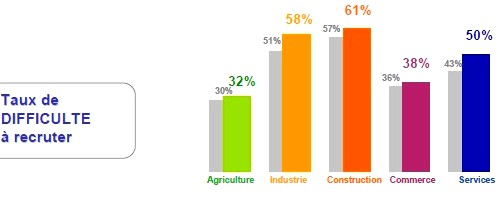
\includegraphics[trim=7cm 0cm 0cm 0cm, clip=true, width=0.5\textwidth]{../resources/illustrations/diff_recrut}
		};
	\end{tikzpicture}
	\includegraphicsabsolute{../resources/illustrations/embauches}{.5\textwidth}{6.5cm}{3cm}
	\footlineextra{\cite{recrutement_midi_pyr}}
\end{frame}


\subsection{Communication}

\begin{frame}{Embauches et internet}
	\includegraphicsabsolute{../resources/illustrations/recrutement-enquete}{.6\textwidth}{0.2cm}{1.7cm}
	\includegraphicsabsolute{../resources/illustrations/online_recrut}{.6\textwidth}{6cm}{3.5cm}
	\footlineextra{\cite{recrutement_internet, recrut_social_network,social_recrut}}
\end{frame}

\begin{frame}{Réseaux sociaux et chantage}
	\includegraphicsabsolute{../resources/illustrations/Amanda_Todd}{.6\textwidth}{0.2cm}{1.7cm}
	\includegraphicsabsolute{../resources/illustrations/facebook_blackmail}{.6\textwidth}{6cm}{4.7cm}
	\footlineextra{\cite{chantage_facebook, harcel_facebook}}
\end{frame}

\subsection{Décrochages et échecs scolaires}

\begin{frame}{Formation inadaptée}
	\begin{tikzpicture}[remember picture,overlay]
		\node[anchor=north west,inner sep=0pt] at ($(current page.north west)+(0.5cm,-1.5cm)$) {
			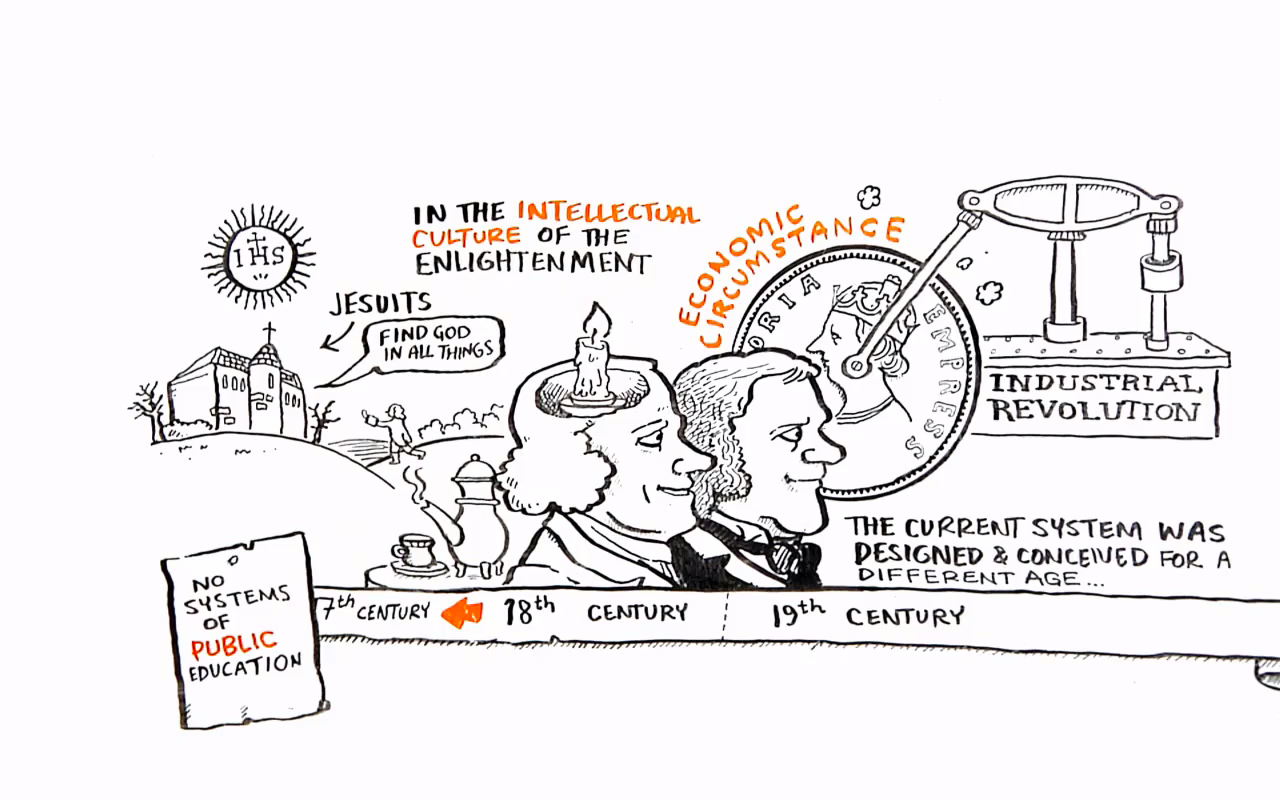
\includegraphics[trim=2cm 1.5cm 0cm 1.5cm, clip=true, width=\linewidth]{../resources/illustrations/public_education}
		};
	\end{tikzpicture}
	\footlineextra{\cite{robinson2010paradigms}}
\end{frame}

\begin{frame}{Troubles de l'attention}
	\begin{tikzpicture}[remember picture,overlay]
		\node[anchor=north west,inner sep=0pt] at ($(current page.north west)+(1.5cm,-1.5cm)$) {
			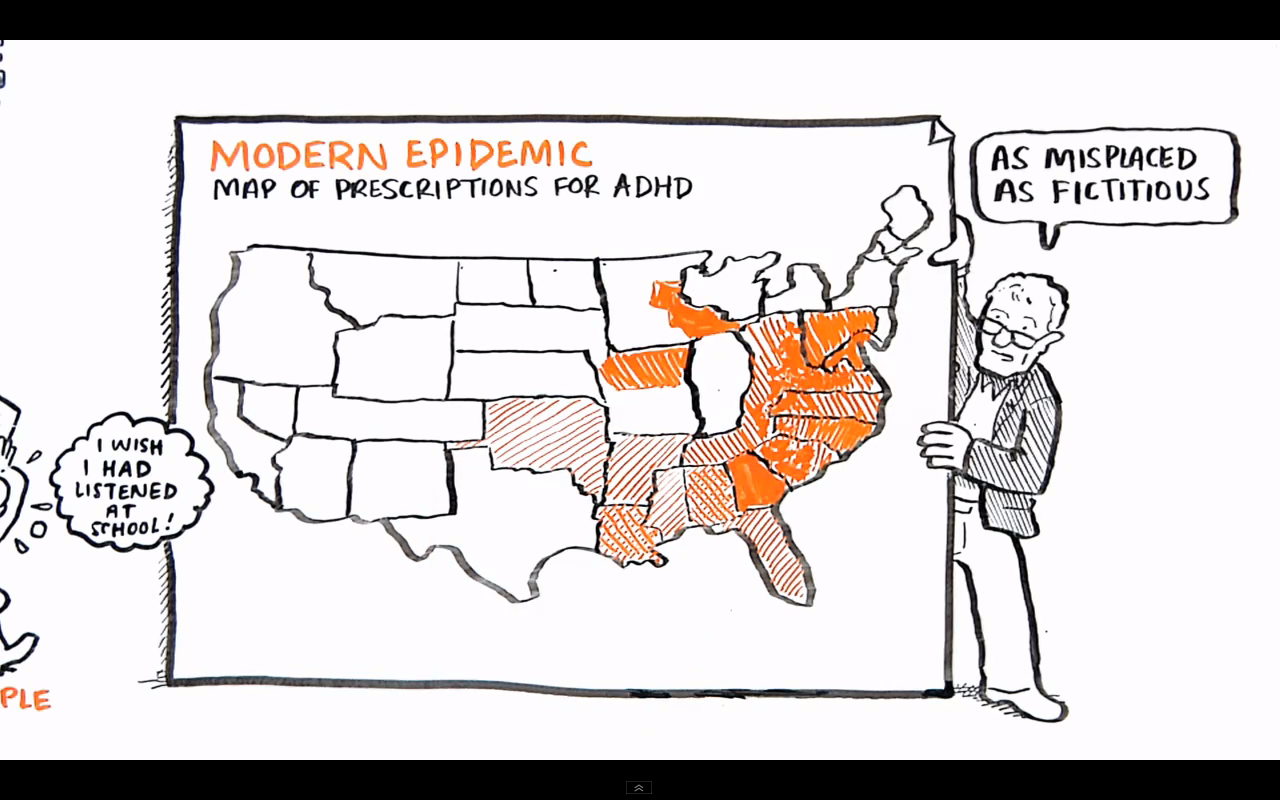
\includegraphics[trim=1.9cm 1.5cm 0cm 1.5cm, clip=true, width=\linewidth]{../resources/illustrations/ADHD}
		};
	\end{tikzpicture}
	\footlineextra{\cite{robinson2010paradigms}}
\end{frame}


